%\documentclass[a4paper,11pt,aas_macros]{report}

\documentclass[usenatbib]{mnras}
%Check if we are compiling under latex or pdflatex
% see e.g. http://www.2pi.info/latex/Includingeps.html
\ifx\pdftexversion\undefined \usepackage{epsf,epsfig}
%  \usepackage[dvips]{graphicx}
\else \usepackage[pdftex]{graphicx} \fi
\usepackage{lscape}
\usepackage{color}
\usepackage{amsmath}
%\usepackage{ulem}
\bibliographystyle{mnras}
%\usepackage[T1]{fontenc}

%%%%%%%%%%%%%%%%%%%%%%%%%%%%
% ANY OTHER DECLARATIONS HERE:
\newcommand{\Herschel}{\textit{Herschel} }
\newcommand{\um}{\micron\  }
\newcommand{\STARFINDER}{{\sc starfinder}}
\newcommand{\DESPHOT}{{\sc desphot}}

%%%%%%%%%%%%%%%%%%%%%%%%%%%%


\title[HELP: The Herschel Extragalactic Legacy Project]{HELP: The Herschel
  Extragalactic Legacy Project\footnote{{\em Herschel} is an ESA space
  observatory with science instruments provided by European-led Principal
Investigator consortia and with important participation from NASA.}}
\date{June, 21st 2018}
\author[S. J. Oliver et al.]
{
  \parbox{\textwidth}
  {\raggedright S.J. Oliver$^{1}$\thanks{S.Oliver@Sussex.ac.uk},
% Project scientists alphabetically
  K.~Duncan,$^{2}$
  P.D.~Hurley,$^{1}$
  K.~Ma\l{}ek,$^{3}$
  R.~Shirley,$^{1,4,5}$
  M.~Vaccari,$^{40}$
% Alphabetically
  H.~Aussel,$^{7}$
  T.~Bakx,$^{20}$
  V.~Buat,$^{10}$
  D.~Burgarella,$^{10}$
  M.C.~Campos~Varillas,$^{1}$
  N.~Christopher,$^{35}$
  S.~Duivenvoorden,$^{1}$
  S.~Eales,$^{20}$
  A.~Efstathiou,$^{35}$
  E.A.~Gonz\'alez~Solares,$^{24}$
  M.~Griffin,$^{20}$
  M.~Jarvis,$^{40}$
%  E.~Le~Floc'h,$^{7}$
  B.~Lo~Faro,$^{21}$
  L.~Marchetti,$^{40}$
  V.~Papadopoulou,$^{35}$
  K.~Penner,$^{7}$
  E.~Pons$^{24}$,
  M.~Prescott,$^{40}$
  E.~Rigby,$^{30}$
  H.~Rottgering,$^{30}$
  Y.~Roehlly,$^{1}$
  J.~Scudder,$^{1}$
  M.~Smith,$^{20}$
  and L.~Wang.$^{2}$
}
\vspace{0.4cm}\\
\parbox{\textwidth}
{\raggedright
  $^{1}$Astronomy Centre, Dept. of Physics \& Astronomy, University of Sussex,
  Brighton, BN1 9QH, UK\\
  $^{2}$Sterrewacht Leiden, Universiteit Leiden, Leiden, Netherlands\\
  $^{3}$National Centre for Nuclear Research, ul. Ho$\dot{z}$a 69, 00-681 Warszawa, Poland\\
  $^{4}$Instituto de Astrof\'isica de Canarias, E-38205 La Laguna, Tenerife, Spain\\
  $^{5}$Universidad de La Laguna, Dpto. Astrof\'isica, E-38206 La Laguna, Tenerife, Spain\\
  $^{7}$Laboratoire AIM-Paris-Saclay, CEA/DSM/Irfu - CNRS - Universit\'e Paris
  Diderot, CE-Saclay, pt courrier 131, F-91191 Gif-sur-Yvette, France\\
  $^{10}$Aix Marseille Univ, CNRS, LAM, Laboratoire d'Astrophysique de Marseille, 
Marseille, France\\
  $^{20}$School of Physics and Astronomy, Cardiff University, Queens Buildings,
  The Parade, Cardiff CF24 3AA, UK\\
  $^{24}$Institute of Astronomy, University of Cambridge, Madingley Road,
  Cambridge CB3 0HA, UK\\
  $^{2}$Netherlands Institute for Space Research, SRON\\
  $^{35}$European University Cyprus\\
  $^{40}$UWC\\
  $^{50}$Stanford\\
}}

%%%%%%%%%%%%%%%%%%%%%%%%%%%%
% BEGIN DOCUMENT
\begin{document}
%\tableofcontents
\maketitle
%%%%%%%%%%%%%%%%%%%%%%%%%%%%


%%%%%%%%%%%%%%%%%%%%%%%%%%%%
\section*{Notes on draft}

{\color{red} This draft 21-June-2018 (updated 6th September 2019) is a rough skeleton for comments by the
team.  Authorship is those who are funded participants, who contributed to the
proposal or have made an additional direct contribution to this paper. All
authors will be expected to provide comments or indicate that they are happy
with content. Authorship order is PI followed by Project Scientists and then
ordered  alphabetically, this may not be the final ordering, hence I've not
bothered sorting the institutional numbers. I was tempted to rip stuff out of
the proposal, but I think that might be too verbose. The table of contents is
obviously just to aid in understanding the structure}

\setcounter{tocdepth}{3}\tableofcontents


\begin{abstract}
  We describe a new project to collate, curate, homogenise and add-value to most 
  of the premium multi-wavelength extragalactic data sets over 1300 ${\rm
  deg}^2$. The sky boundaries of \Herschel Extragalactic Legacy Project, HELP, 
  are currently defined by almost all of the \Herschel SPIRE extragalactic survey fields,
  notably the \Herschel Multi-tiered Extragalactic Survey (HerMES) and the
  \Herschel Atlas survey (H-ATLAS). HELP brings together data at all wavelengths
  from radio to X-ray.  This paper describes the motivation and the principle
  elements in the design of the project. Guiding principles are transparent or 
  ``open" methodologies with care for reproducibility and identification of provenance. 
  A key element of the design focuses
  around the homogenisation of calibration, meta data and the provision of
  information required to define the selection of the data in fashion that 
  they can be used for statistical analysis. This goes significantly beyond 
  what is available in standard virtual observatory protocols. The full
  scientific exploitation of this requires novel methods.  We  advocate
  probabilistic methods that extract information directly from the maps at long
  wavelengths, exploiting the prior information available at shorter wavelengths
  and providing full sampling of the posteriors rather than traditional
  catalogues. 
With this project definition paper we provide full access to the first data release of HELP (DR1),
including a monolithic map of the largest SPIRE extragalactic
  field at 385 deg$^2$, XXX PACS and SPIRE fluxes across YYY sq.deg. We also provide tools to access the
  information currently in the HELP database. All software used for processing the data is publicly available on GitHub.  
\end{abstract}

\begin{keywords}
  techniques: photometric -- catalogues -- surveys -- infrared: galaxies --
  submillimetre: galaxies -- galaxies: evolution
\end{keywords}
%-----------------------------------------------------
% Chapter
%-----------------------------------------------------
\section{Introduction}\label{sec:intro}


A fundamental requirement for rigorous testing of any theories of galaxy
formation and evolution is a complete statistical audit or census of the stellar
content and star formation rates of galaxies in the Universe at different times
and as a function of the mass of the dark matter halos that host them.

This audit requires many elements.   We need un-biased maps of large volumes of
the Universe made with telescopes that probe the different wavelengths at which
the different physical processes of interest manifest themselves. We need
catalogues of the galaxies contained within these maps with photometry estimated
uniformly from field-to-field, from telescope-to-telescope and from
wavelength-to-wavelength. We need to understand the probability of a galaxy of
given properties appearing in our data sets.  We need the machinery to bring
together these various data sets and calculate the ``value-added" physical data
of primary interest, e.g. the distances, stellar masses,
star-formation rates and the actual number densities of the different galaxy
populations.

For decades many  teams  have been undertaking ambitious coordinated
multi-wavelength programmes to study large volumes of the distant Universe.
These surveys are now becoming sufficiently complete that we are now able to
undertake the necessary homogenising and adding value and thus provide the first
representative and comprehensive census of the galaxy populations in the distant
Universe.

Collation of multi-wavelength data has been undertaken for very deep surveys
over small areas (less than few deg$^2$) in particular COSMOS\citep{cosmos} and ASTRODEEP\citep{astrodeep} and
for wide nearby surveys (over 200-1000 deg.$^2$) especially SDSS\citep{sdss} and GAMA\citep{gama}.
However, due to size of the data and complexity arising from the variety of
observatories required little concerted effort has been made to assemble the
deep surveys over 10-1000 deg.$^2$. These surveys are particularly important as
they are large enough to probe representative  ranges of environments and to
provide large statistical samples to  fully explore the range of galaxy
phenomena in detail and including rare, transitory phenomena.

ESA's {\em Herschel}\citep{pilbrat} mission has a unique role in these studies, probing the
obscured star-formation activity, which at high redshifts forms about 80\% of
all star formation The {\em Herschel} extra-galactic surveys were a major goal
of {\em Herschel} and occupied around 10\% of the {\em Herschel} mission.  These
surveys cover enough of the sky to provide representative samples of dark matter
halos including the most massive ones.

The {\em Herschel} SPIRE instrument is sufficiently sensitive that the maps can
detect most ($>60\%$) of the emission making up the cosmic infra-red background
radiation (CIBR), which itself makes up roughly half of the total background
radiation from galaxies.  However, the large beam size means that the objects
that can be clearly seen as individual sources only make up about 15\% of the
CIBR.  A particular focus of our HELP is to employ new methods to learn from our
large statistically meaningful samples the relationship between the ancillary
data  and the {\em Herschel} data and thus unlock the full information from the
{\em Herschel} maps and then make that available as a legacy to the community.

The final pieces of this multi-wavelength survey programme will be completed
with the optical, NIR and radio surveys being carried out during the lifetime of
this grant.  The VISTA near-infra-red surveys detect the radiation from the old
stellar population in galaxies, which accounts for most of the stellar mass,
while the radio surveys being carried out the next few years with LOFAR, MeerKAT
and ASKAP detect radiation associated with the young stellar population and with
AGN.

Statistical modelling of galaxy populations requires a detailed understanding
and modelling of the selection processes in the basic data products and the
derived properties.   These ``selection functions'' are seldom available for
individual data sets and rarely, if ever, published for derived physical
properties.  We will produce these and make them all public.

A key motivation of large area surveys is to probe galaxy populations in all
environments. Cluster catalogues and density maps are only really possible with
the homogeneous multi-wavelength data over wide fields we will have provided. So,
we will provide these to the community.

The techniques, tools and data we provide will enable astronomers in Europe to
fully capitalise on resources provided by {\em Herschel} and the other surveys,
extending the kinds of scientific investigation possible a decade ago in the
nearby Universe with the SDSS into the early Universe and providing a lasting
legacy for surveys and facilities in the future.  

This paper presents the HELP. In Section~\ref{sec:fields} we describe the define
the HELP fields.   In Section~\ref{sec:surveys} we describe . In
Section~\ref{sec:metrics} we provide metrics of the catalogue quality by
injecting synthetic sources.   In Section~\ref{HeLMSextended} we discuss
extended sources and artefacts. In Section~\ref{sec:catcomp} we compare with
similarly constructed catalogues of Herschel sources in the  HerS field
\cite{Viero:2014lr}, a 79 deg$^2$ field which has a 10 deg$^2$ overlap.  We
discuss the uses of this catalogue and future work in
Section~\ref{sec:discussion} and conclude in Section~\ref{sec:conclusions}.


\section[The HELP fields.  
\\
{\color{red}A section that copies the figure used in Raph's paper, but goes into more detail about the nature of each of the fields, e.g. with the percentiles of dust intensities from the Planck maps and provides the definitive MOCs for the (DR1) survey boundaries (electronically)}]
{The HELP fields}\label{sec:fields}

Many extragalactic surveys from different observatories and different
wavelengths have been coordinated in their planning and execution. However, many
had different motivations and all had different factors constraining their
choice of field locations and sizes. So, to define a common boundary is
a challenge.  Nevertheless to collate a set of data we need to define some rigid
boundaries. Given that there is no imminent successor to  \Herschel  the data
from that mission provides a legacy benchmark.  Within the \Herschel observatory
the SPIRE instrument \citep{Griffin:2010lr} mapped larger areas than the PACS
instrument \citep{Poglitsch:2010lr}. We thus decided to define the boundaries of
the project on the basis of the extra-galactic surveys carried out with SPIRE.
The specific \Herschel OBSIDS chosen to define the project are listed in
Appendix~\ref{sec:obsids}

The \Herschel Multi-tiered Extragalactic Survey (HerMES, \citealt{Oliver:2012})
is a major survey conducted by the \Herschel mission\citep{Pilbratt:2010lr}
using the SPIRE \citep{Griffin:2010lr} and PACS \citep{Poglitsch:2010lr}
instruments.  The largest and shallowest of the HerMES SPIRE fields, making up
the bottom of the ``tiered wedding cake''  is the HerMES Large Mode Survey,
HeLMS.

\begin{table*}
  \begin{tabular}{|l|r|r|r|r|r|r|r|}
\hline
  \multicolumn{1}{|c|}{Name} &
  \multicolumn{1}{c|}{RA} &
  \multicolumn{1}{c|}{Dec} &
  \multicolumn{1}{c|}{RA min} &
  \multicolumn{1}{c|}{RA max} &
  \multicolumn{1}{c|}{Dec min} &
  \multicolumn{1}{c|}{Dec max} &
  \multicolumn{1}{c|}{Area} \\
  \multicolumn{1}{|c|}{} &
  \multicolumn{1}{c|}{[deg]} &
  \multicolumn{1}{c|}{[deg]} &
  \multicolumn{1}{c|}{[deg]} &
  \multicolumn{1}{c|}{[deg]} &
  \multicolumn{1}{c|}{[deg]} &
  \multicolumn{1}{c|}{[deg]} &
  \multicolumn{1}{c|}{[deg.$^2$]} \\
\hline
  SSDF & -8.1 & -55.1 & -357.8 & -18.5 & -60.5 & -48.5 & 110.4\\
  HATLAS-SGP & 1.5 & -32.7 & 337.2 & 26.9 & -35.6 & -24.5 & 294.6\\
  ELAIS-S1 & 8.8 & -43.6 & 6.4 & 11.2 & -45.5 & -41.6 & 9.0\\
  Herschel-Stripe-82 & 14.3 & 0.0 & 348.4 & 36.2 & -9.1 & 8.9 & 363.4\\
  XMM-LSS & 35.1 & -4.5 & 32.2 & 38.1 & -7.5 & -1.6 & 21.8\\
  CDFS-SWIRE & 53.1 & -28.2 & 50.8 & 55.4 & -30.4 & -26.0 & 13.0\\
  AKARI-SEP & 70.8 & -53.9 & 66.2 & 75.4 & -55.9 & -51.7 & 8.7\\
  GAMA-09 & 134.7 & 0.5 & 127.2 & 142.2 & -2.5 & 3.5 & 62.0\\
  COSMOS & 150.1 & 2.2 & 148.7 & 151.6 & 0.8 & 3.6 & 5.1\\
  Lockman-SWIRE & 161.2 & 58.1 & 154.8 & 167.7 & 55.0 & 60.8 & 22.4\\
  GAMA-12 & 179.8 & -0.5 & 172.3 & 187.3 & -3.5 & 2.5 & 62.7\\
  HDF-N & 189.2 & 62.2 & 188.1 & 190.4 & 61.8 & 62.7 & 0.67\\
  SA13 & 198.0 & 42.7 & 197.6 & 198.5 & 42.4 & 43.0 & 0.27\\
  HATLAS-NGP & 199.5 & 29.2 & 189.9 & 209.2 & 21.7 & 36.1 & 177.7\\
  XMM-13hr & 203.6 & 37.9 & 202.9 & 204.4 & 37.4 & 38.5 & 0.76\\
  EGS & 215.0 & 52.7 & 212.4 & 217.5 & 51.2 & 54.2 & 3.6\\
  GAMA-15 & 217.6 & 0.5 & 210.0 & 225.2 & -2.5 & 3.4 & 61.7\\
  Bo\"otes & 218.1 & 34.2 & 215.7 & 220.6 & 32.2 & 36.1 & 11.4\\
  ELAIS-N1 & 242.9 & 55.1 & 237.9 & 247.9 & 52.4 & 57.5 & 13.5\\
  ELAIS-N2 & 249.2 & 41.1 & 246.1 & 252.3 & 39.1 & 43.0 & 9.2\\
  xFLS & 259.0 & 59.4 & 255.6 & 262.5 & 57.9 & 60.8 & 7.4\\
  SPIRE-NEP & 265.0 & 69.0 & 263.7 & 266.4 & 68.6 & 69.4 & 0.6\\
  AKARI-NEP & 270.0 & 66.6 & 264.6 & 275.3 & 64.5 & 68.5 & 9.2\\
\hline\end{tabular}

  \caption{Summary of HELP fields.  The total area is 1269.1 deg.$^2$}
\end{table*}


\begin{figure*}
  \centering 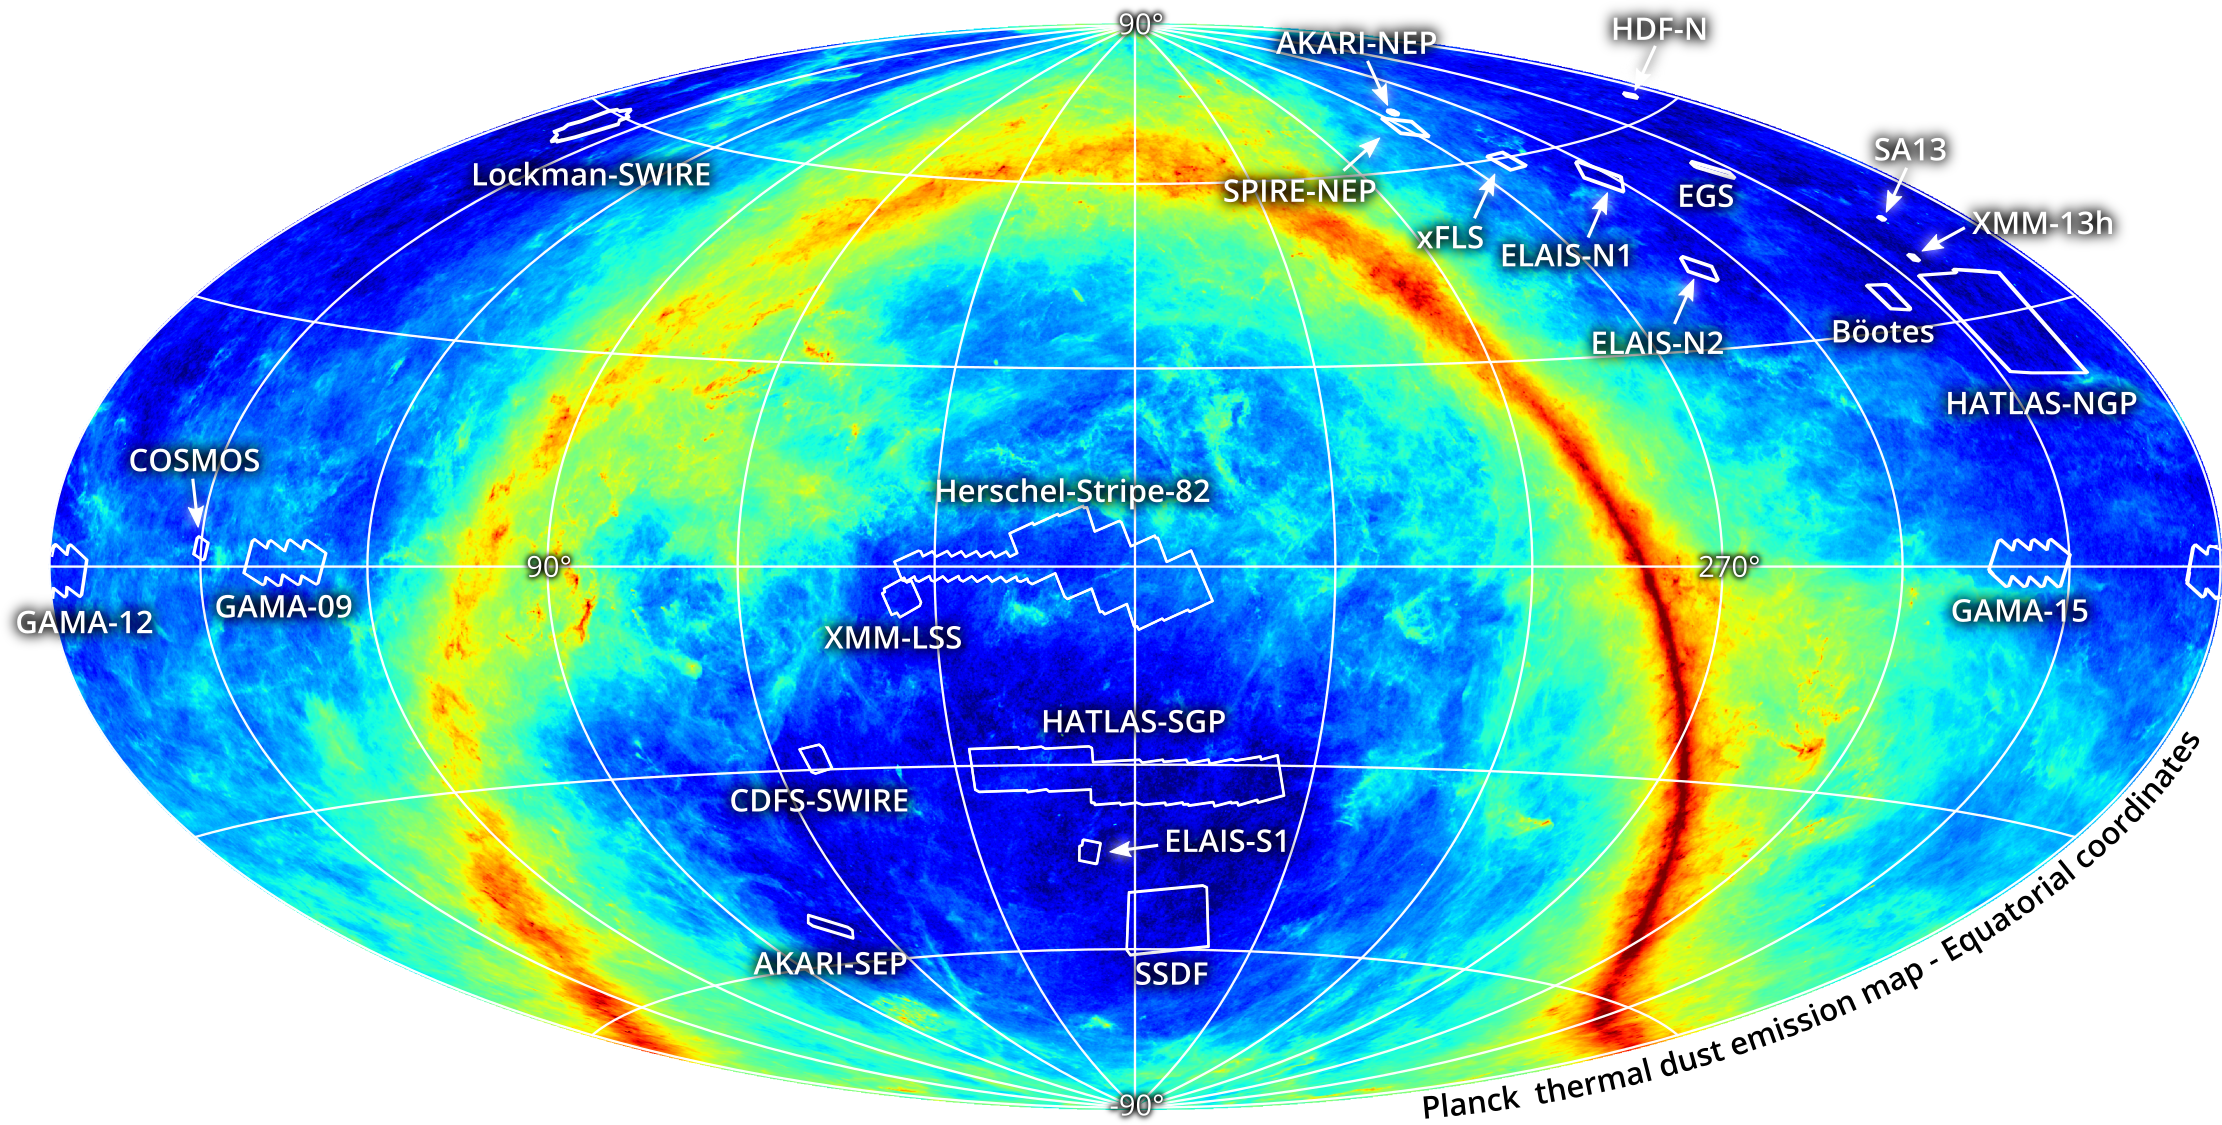
\includegraphics[width=16cm]{figs/HELP-fields.png}
  \caption[HELP Sky]{Projection of the HELP fields onto the dust emission from
    our own Galaxy. Reproduced from \citet{Shirley:2019}}.\label{fig:helpsky}
\end{figure*}


%Raph - removed this because we have covered opt-nir depths in Shirley et al
%Adding 2d and MIPS + depths in its place.
%\begin{figure}
%  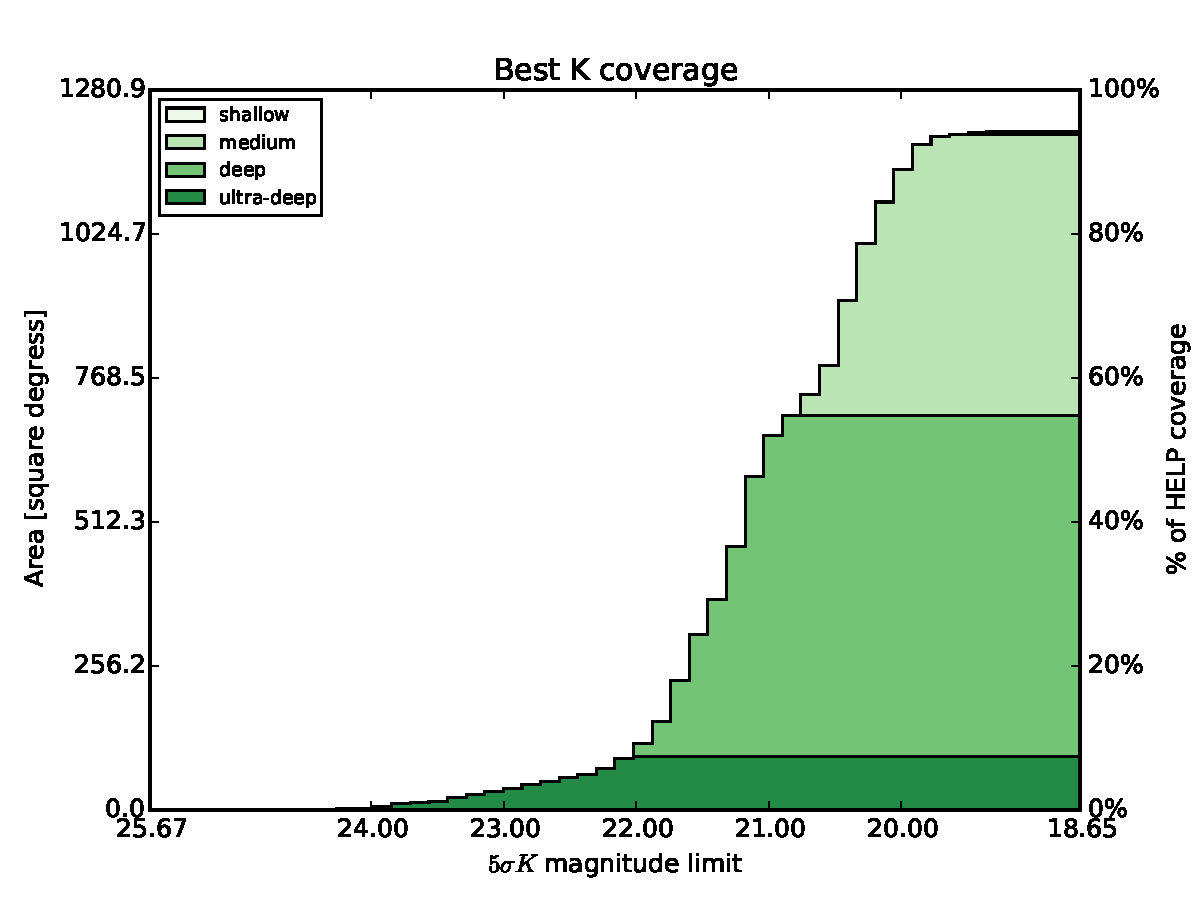
\includegraphics[width=8cm]{figs/K_coverage_v1_2_full.pdf}
%  \caption[K-band coverage]{The cumulative area within HELP covered to a given
%    $K_{\rm AB}$ depth. In this case the depth has been defined using the
%    $\sigma$ from the flux errors of objects in the catalogues. This is an example
%    of the summary report that can be generated from the HELP database. Similar
%    plots can be generated for other bands, over individual fields and jointly
%    limiting in more than one band. }\label{fig:k}
%\end{figure}

\begin{figure*}
  \centering 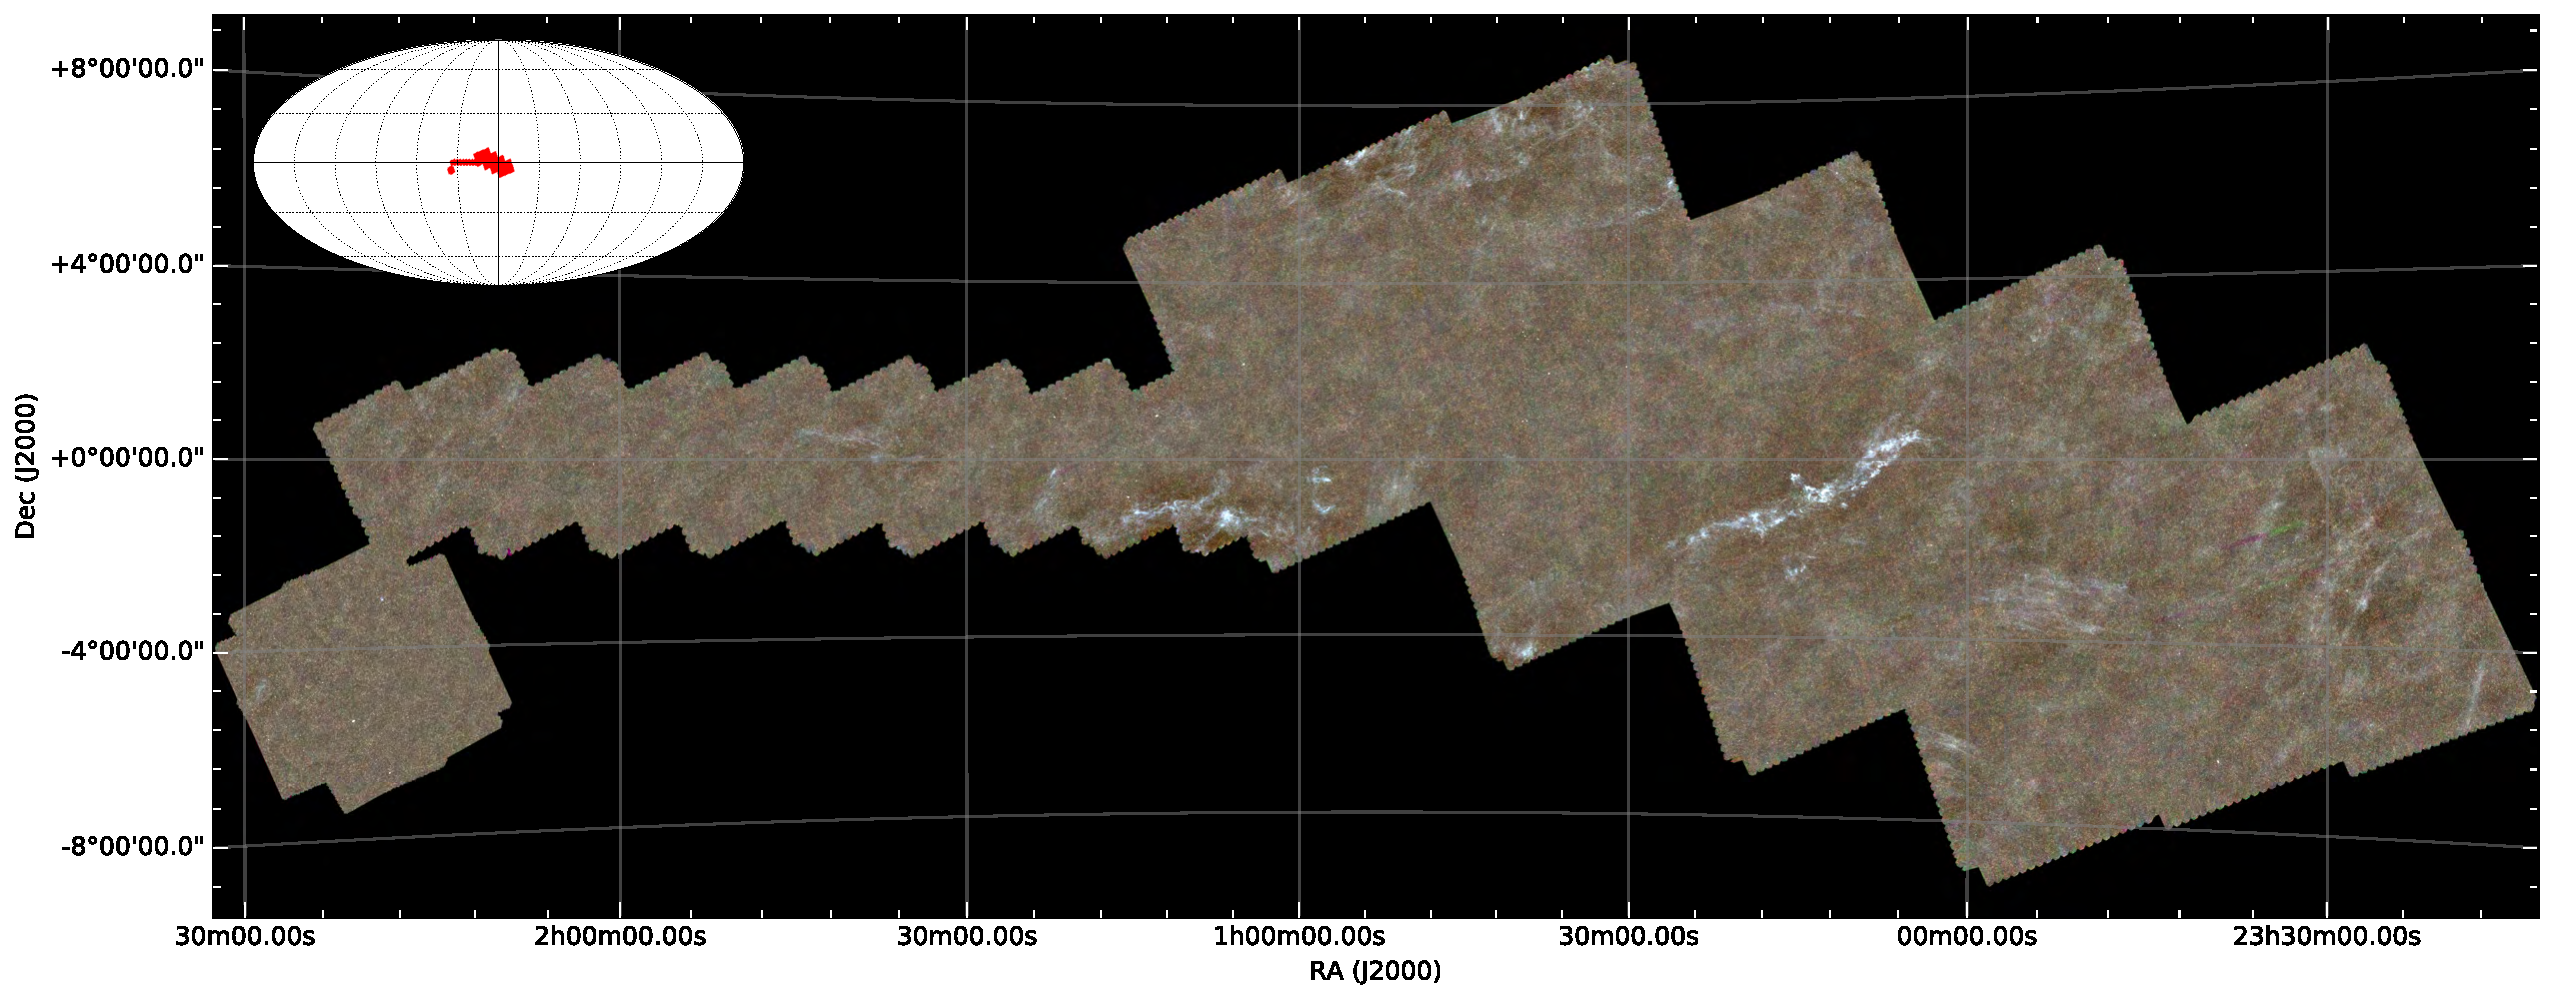
\includegraphics[width=16cm, angle=0]{figs/helms_hers_xmm-lss-rgb-sm.pdf}

  \caption[Three-colour image of Herschel Strip 82 region]{RGB representation of
    the Herschel Stripe 82 and XMM-LSS field, with 250\um, 350\um and 500\um
    represented by blue, green and red respectively. This is the largest
    contiguous extra-galactic region observed by \Herschel\.  The maximum scale
    of the field from the East to West tips is  50\degr and the separation from
    edge-to-edge (following the zig-zag, roughly North-to-South) is 11\degr. The
    inset indicates the location of this region on an all-sky equatorial
    projection. The total area of  this field is 385 deg.$^2$. Readily apparent
    is the strong cirrus structure throughout the map, including a ``seagull"
    like shape in the centre.  The data comes from three different observations
    (XMM-LSS, HELMS from HerMES \citealt{Oliver:2012} and the HERS. This maps
    was built for HELP from the processed SPIRE time-lines using the HerMES SMAP
    processing.}\label{fig:hs82}
\end{figure*}

\subsection[The multi-wavelength surveys.\\ 
{\color{red} This refers to the summary in optical NIR in Raph's paper but lists also the other surveys (i.e. at UV, X-ray, mid-IR, FIR, sub-mm and Radio) and whether or not they are included in DR1.  It might be sensible to merge this with the previous section}]{The multi-wavelength surveys.}\label{sec:surveys}

The first stage of the HELP pipeline is to build a catalogue of auxiliary optical to mid infrared catalogues that combine to make the prior list for extraction of far-infrared fluxes. This positional cross match of over 50 public surveys is described in detail in \citep{Shirley:2019} and the process is summarised in section~\ref{sec:masterlist}. Here we summarise the various input data sets and their overall depths.


\subsubsection[The depth of data\\
{\color{red} (no longer needed as this is now a separate paper, but Intro might refer to this paper and subsequent DR1 results sections might relate to this). A section to look at CIRB vs mag and the co-variances of the
multi-wavelength data }]{The depth of data}

The depths of the input catalogues are of crucial importance in determining the depth of fluxes extracted from the far-infrared red maps. They also determine the depths and completeness of photometric redshifts and must be properly accounted for in building statistical samples of galaxies.



\section[HELP Strategy \\
{\color{red} This Section will cover things that are related to the overall HELP philosophy and strategy that include, but go beyond DR1}]{HELP Strategy}
{\color{red} This Section will cover things that are related to the overall HELP philosophy and strategy that include, but go beyond DR1}

HELP is designed to create a framework for wide area multiwavelength studies. In this first data release DR1 this is heavily determined by regions on the sky where the \emph{Herschel} SPIRE instrument observed deep extragalactic fields. In this paper we are presenting this first data release but also the software, tool, and other resources to move beyond the first release and be continuously updated with new deeper observations. Further, the aim is to provide tools to create statistically useful samples of objects taking into account the quality and features of the presently available data. 

\subsection{Homogenisation}

At the most basic level this means providing homogeneous data products in terms of measures, units, and data formats.

\subsection{Meta data}

The data presented here has been compiled with extensive meta data available. In order to aid the user in compiling references and other tasks, we have spent considerable effort in providing written descriptions of all the data in addition to machine readable files with links to papers, summaries of coverage and descriptions of instruments, including definitions of bands and links to transmission curves.

\subsection{Selection Functions}

The selection function is the probability of a galaxy being detected and included as a function of the galaxy properties. Determining the form of these functions is a major challenge over wide areas of the sky. In dedicated surveys it is common to construct, for instance, magnitude limited samples in an attempt to create as simple a selection function as possible. Here, we are collating previous surveys and so cannot determine survey design. We therefore need to develop tools to reverse engineer the selection function. A simple application of such a selection function could be for example: determine the volume over which a given object would be detected and present in the sample such that the objects density in the Universe can be estimated. This is crucial for producing empirical summaries of populations such as luminosity functions. The following list describes some selections functions at varying levels of sophistication:

\begin{itemize}
  \item{Binary coverage:} Multi-Order Coverage maps, MOCs
  \item{Depth maps:} Multi-Order Depth maps, MODs
  \item{Completeness Curves:} Multi-Order Logistic Curves MOLCs. Based on
    logistic curve parameters, but also in multi-order
  \item{Full likelihood function:} The probability of a given galaxy being detected at a given redshift and position on the sky.
\end{itemize}


\subsection[Forced photometry\\ {\color{red} not done in DR1 so some discussion}]{Forced photometry}

With high resolution data we will provide photometry either by matching
catalogues or by returning to the images and extracting the photometry if the
original catalogues do not include the photometric data we require.
\subsection[Blind catalogues, cross-matching and supplementary lists\\{\color{red}Some of this should go into the strategy as it is not implemented in DR1, but this is where to discuss the blind SPIRE catalogues that Steven has produced, plus spec-z catalogues, radio catalogues?}]{Blind catalogues, cross-matching and supplementary lists}

\subsection[Open Science]{Open Science}
The project has been implemented using open science frameworks. This has been achieved with the following general 



\subsection{Tools}

The philosophy with HELP is that we should be providing the data, meta data and
tools such that astronomers can easily carry out their scientific investigations
without a high level of instrument or survey-level expertise.  We have defined
some specific scientific use-cases which should be achievable at the end of the
project.  These are aimed to result in recipes at the level  that a postgraduate
student (under the supervision of an astronomer) could take and produce
meaningful scientific results.  Our intention is that all scientific results
from the team could be easily reproduced using these tools.  We anticipate that
some of these tools will be database operations.  Our database is VO enabled
with ADQL interfaces.  Some tools will be traditional client/server interfaces.
Other tools will be developed to provide containers (e.g. Docker) that the user
can down-load and run on their own CPU resources.  All software will be made
open source and distributed through public repositories (e.g. GIThub).

\section{The DR1 work-flow}[The DR1 work-flow\\{\color{red} A section to define the HELP pipeline as used in DR1.  }]
{\color{red} A section to define the HELP DR1 pipeline.  }

In this section we describe the photometry work-flow.  We create a master list 
of astronomical sources and collate photometry measurements for these sources 
at all wavelengths. Part of this process involves determining the highest 
quality measurements available in a given field and wavelength region. In order 
for subsequent data processing to work effectively, there should be high quality 
photometry across a wide spread of wavelengths. This stage also allows us to 
investigate the depths available in a given area for a given band. Obviously,
some of the fields in the HELP areas have more high quality surveys available than others.
By using Jupyter notebooks to document all the processing on GitHub, all this 
information about data quality is readily available and the code could be rerun with future 
additional survey data. The forced photometry performed by XID+ takes the master list as a hard positional prior. This is then used to provide a further catalogue of far infra red flux measurements.


Brief overview of the whole thing, before going into the details 

\subsection[Master List\\ {\color{red}Basically a very brief summary of Raph's paper, but really just pointing to it}]{Master list}
\label{sec:masterlist}
The HELP master list is contains optical, NIR and IRAC catalogues.  The production of the 
\emph{masterlist} is described in detail in \citep{Shirley:2019}. It includes every 
source with a measurement in at least one band. A positional cross match is then
used to combine the various wavelengths and all sources are flagged to specify
which regions it has measurements as well as whether it was in an area covered by a
given band. Therefore, if the object was not detected in some band and we have a measure 
of the depth available in that band, we have a measure for an upper limit for the flux in
that band. We also provide a table of the original catalogue ids and the original catalogues.
This means that where additional useful information is included in the input catalogue,
it can be quickly recovered using the table of cross identifiers. All this data is provided in a
simple and well documented structure to facilitate independent validation and external use.
{\color{red} outline of the work-flow to (a) define the master list, (b) reject
spurious sources including artefacts and those around bright stars stars (c)
classification of sources }

The \emph{masterlist} is used to compute photometric redshifts.

\begin{itemize}
  \item{Baseline: point list}
  \item{Silver: point list, with size and shape}
  \item{Gold: two component shape model (bulge and disk)}
  \item{Platinum: full morphological description e.g. based directly on
    short-wavelength image}
\end{itemize}

\subsection[Prior catalogue and model\\{\color{red}Describing how we define the different prior lists in each field/area}]{A prior catalogue and model}

{\sc XID+} is designed to accept a general prior probability on the flux of each object. The following gives an overview of the priors that it is possible to employ:

\begin{itemize}
  \item{positional priors}
  \item{flux priors}
  \item{observed colour priors}
  \item{redshift, SED priors}
  \item{luminosity/environment priors}
\end {itemize}

For some science purposes it is useful to employ informative priors based on all the information available for a given source. For HELP, due to the widely varying data available on a given patch of sky we decided to employ a general prior which does not take account of the full multiwavelength flux values. 

\subsection{\emph{XID+}: the probabilistic deblender for confusion dominated maps}
For many of our fields, in addition to the SPIRE maps we also have Spitzer MIPS $\mathrm{\mu m}$ and Herschel PACS 100 and 160 $\mathrm{\mu m}$ maps that cover the mid to far-infra-red part of the electromagnetic spectrum. However, due to the relatively large beam size of the these maps compared to the galaxy density ($\approx 30$ per SPIRE beam for optical sources with $B < 28$), multiple galaxies can be located within the instrument beam. This is referred to as the problem of source confusion.

To obtain accurate photometry from these infra-red maps, overcoming the source confusion problem is essential. One way to solve the problem is to use prior information to accurately distribute the flux in the maps to the underlying astronomical objects. For example, if we know the location of a galaxy to a reasonable tolerance (e.g. from an optical image where resolution is better), we may expect a galaxy to be found in the MIPS, PACS and SPIRE maps at the same location.

As part of HELP, we have developed \emph{XID+} \citep{Hurley:2017} which uses a probabilistic Bayesian approach that provides a natural framework in which to include prior information and obtain the full posterior probability distribution on flux estimates. Obtaining the full posterior probability distribution is particularly important for getting accurate uncertainties on source flux.

\subsubsection[HELP XID+ pipeline \\ {\color{red}Discusses how this was applied for different bands and prior lists}  ]{HELP XID+ pipeline}
HELP uses XID+ to carry out forced photometry on the Spitzer MIPS, Herschel PACS and Herschel SPIRE maps. As the output fluxes are products for the main database, we stick to positional and uninformative flux priors (i.e. uniform flux prior) to enable the widest range of analysis with the HELP data products. Additional prior information is a powerful approach to get more out of the data, however their use must be fully understood and taken into account when carrying out further analysis. For example, the fluxes coming from a version of XID+ that uses SED templates as a prior, cannot then be used to fit SEDs with a different set of templates. We have explored numerous ways of adding additional prior information and provide these as part of the XID+ software package for users to carry out their own sophisticated fitting on their chosen sources. 

Our list of prior sources are constructed from the master list, described in Section \ref{sec:masterlist}. Ideally, we would use all sources in the master list as our prior list. In reality, there are too many sources to constrain from the data, unless one goes to more informative priors. We therefore cut down the master list to sources detected in bands that are good tracers of infrared emission, such as K band or IRAC \citep{Duivenvorden:2018}. For fields covered by Spitzer, we use sources detected in any of the Spitzer IRAC bands. To remove any possible artefacts in the IRAC catalogues, We impose an additional constraint that sources must also have a detection in either the optical or NIR wavelength range (using the $opt_nir_det$ flag). 

Across all HELP we define a prior for {\sc XID+} objects that is zero for some objects and flat between zero and the pixel value for obejcts that are in the `prior list'. The factors determining whether an object is in the list depend on the area of sky. For areas that have been surveyed by the \emph{Spitzer} IRAC i1 band an object is in the prior list if it is detected in IRAC i1 and has at least two optical detections and at least two NIR detections. For areas that have not been observed by IRAC i1, we first compute a total dust luminosity for each object using the CIGALE code. An object is then in the prior list if its predicted dust luminosity is above {\color{red} $10^{8.5}$. Need to check units}.


%IRAC prior, selection function, opt_nir_detection, MIPS detection, notebooks
%flag
\subsubsection{HELP XID+ data products}

For each object in the prior list \smallcaps{XID+} provides a posterior on the object flux in each of the \emph{Herschel} bands available. This posterior is given in the form of a sample of 2000 values which, if STAN is converged, should be sampled from the ture posterior. We summarise this in the form of a median, and error. This obviously assumes the posterior is Gaussian. However, we also provide the full posterior which could be used to check this or look for objects where fluxes are correlated with nearby objects. The medians and errors are used by the physical modelling. For individual objects of interest the full posterior and p-value maps (probabilistic residual maps) can be used to verify the quality of the fit. The final data product is a catalogue for each field with these summaries of the posterior for each object.



\subsubsection{XID+ extensions}

%reason for full prob dist. e.g. DESPHOT
%: Pipeline for HELP: explanation for not going beyond positional priors
%Products: marginalised catalogues, Bayesian P-value maps, software to re run and obtain full posterior 
%Additional extensions: CIGALE, full SED

\subsection[Blind catalogues, cross-matching and supplementary lists\\{\color{red}Some of this should go into the strategy as it is not implemented in DR1, but this is where to discuss the blind SPIRE catalogues that Steven has produced, plus spec-z catalogues, radio catalogues?}]{Blind catalogues, cross-matching and supplementary lists}

An essential step in achieving the latter goals and for providing a legacy data
set, suitable for community exploitation is to construct a catalogue of objects
detected in the SPIRE maps without reference to any other data and with fluxes
extracted at the SPIRE wavelengths (a `blind" catalogue).  These catalogues give
a perspective of the sub-mm sky unaffected by any prior prejudice. One
significant challenge is the large SPIRE beam, leading to source confusion (e.g.
\citealt{Nguyen:2010lr}) which requires careful de-blending and the resultant
catalogues of sources do not necessarily correspond one-to-one to individual
galaxies.   To enable statistical studies key metrics for these catalogues are
required to assess: positional and flux biases and accuracy; completeness and
reliability.   Similar catalogues and metrics have been produced and made public
for the other HerMES fields \citep{Smith:2012lr,Wang:2013lr}. A particular
challenge for HeLMS is the high level of emission (``cirrus") from our own
Galaxy.

\subsection[Photometric redshifts\\{color{red} A summary of Ken's paper(s) and any details of exactly what is done for DR1 that is not included in those.}]{Photometric redshifts}

Photometric redshifts are computed using the method presented in \citep{Duncan:2017, Duncan:2018}. For the fields HDF-N, SA13, xFLS, and XMM-13hr we use the photometric redshifts presented in \cite{Zou:2019} based on Legacy Survey $grz$ fluxes and Wise W1, and W2.

\subsection[Physical Modelling\\{color{red} A summary of Kassia's paper(s) and any details of exactly what is done for DR1 that is not included in those.}]{Physical Modelling}

Physical modelling was conducted using the CIGALE code. The full methodology has been described for the ELAIS-N1 pilot field in \citep{Malek:2018}.



\subsection[Database\\{color{red} needs some thought.}]{Database}
All of the data is served at both the Herschel Database At Marseille (HeDAM) and mirrored at the Virtual Observatory at susseX (VOX).




\section[Results\\ {\color{red}Being an assessment of the size and quality of the DR1 product, depths, areas, numbers of sources and redshifts distributions, etc.} ]{Results}

Table~\ref{table:dr1_overview} gives an overview of the numbers of processed objects and areas associated with each field. All fields except the ecliptic poles have been fully processed through the HELP pipeline.

\begin{table*}
%\centering
\caption{Summary of the HELP catalogue in each field. 0 indicates that this aspect of this field is not included in DR1. {\color{red} AS AT 20191010 - rerun with final values. what else should we include? depth measures? aim: All fields except the ecliptic poles have been fully processed for DR1.}}

\label{table:dr1_overview}
\begin{tabular}{l rrrrr}
\hline
Field                & objects    & area deg.$^2^$   & xid+      & photoz    & cigale  \\
\hline
AKARI-NEP            &    531 746 & 9.2              & 35319     & 0         & 0       \\
AKARI-SEP            &    844 172 & 8.7              & 211453    & 0         & 0       \\
Bootes               &  3 481 661 & 11               & 495159    & 1657470   & 38660   \\
CDFS-SWIRE           &  2 171 051 & 13               & 240489    & 139532    & 9308    \\
COSMOS               &  2 599 374 & 5.1              & 44310     & 694478    & 15747   \\
EGS                  &  1 412 613 & 3.6              & 0         & 1183490   & 0       \\
ELAIS-N1             &  4 026 292 & 14               & 120282    & 2885116   & 49986   \\
ELAIS-N2             &  1 783 240 & 9.2              & 86591     & 120961    & 6798    \\
ELAIS-S1             &  1 655 564 & 9.0              & 194276    & 1102319   & 25393   \\
GAMA-09              & 12 937 982 & 62               & 1386659   & 8834023   & 130293  \\
GAMA-12              & 12 369 415 & 63               & 1099477   & 8591676   & 108139  \\
GAMA-15              & 14 232 880 & 62               & 1236395   & 10109159  & 117234  \\
HDF-N                &    130 679 & 0.67             & 0         & 7451      & 0       \\
Herschel-Stripe-82   & 50 196 455 & 363              & 76084     & 21613821  & 0       \\
Lockman-SWIRE        &  4 366 298 & 22               & 242065    & 1382438   & 46719   \\
NGP                  &  6 759 591 & 178              & 1233547   & 3175339   & 185290  \\
SA13                 &      9 799 & 0.27             & 0         & 2891      & 0       \\
SGP                  & 29 790 690 & 295              & 3511594   & 17057212  & 352804  \\
SPIRE-NEP            &      2 674 & 0.13             & 0         & 0         & 0       \\
SSDF                 & 12 661 903 & 111              & 0         & 9268783   & 0       \\
xFLS                 &    977 148 & 7.4              & 52187     & 101282    & 0       \\
XMM-13hr             &     38 629 & 0.76             & 0         & 10777     & 0       \\
XMM-LSS              &  8 705 837 & 22               & 287599    & 6152920   & 61892   \\
\hline
Totals:\\
Percentages:
\hline


\end{tabular}
\end{table*}


Figure~\ref{fig:numbers_allfields} shows the differential number counts in the \emph{Herschel} bands PACS 100, PACS 160, SPIRE 250, SPIRE 350, and SPIRE 500.

\begin{figure*} %[h]
\centering
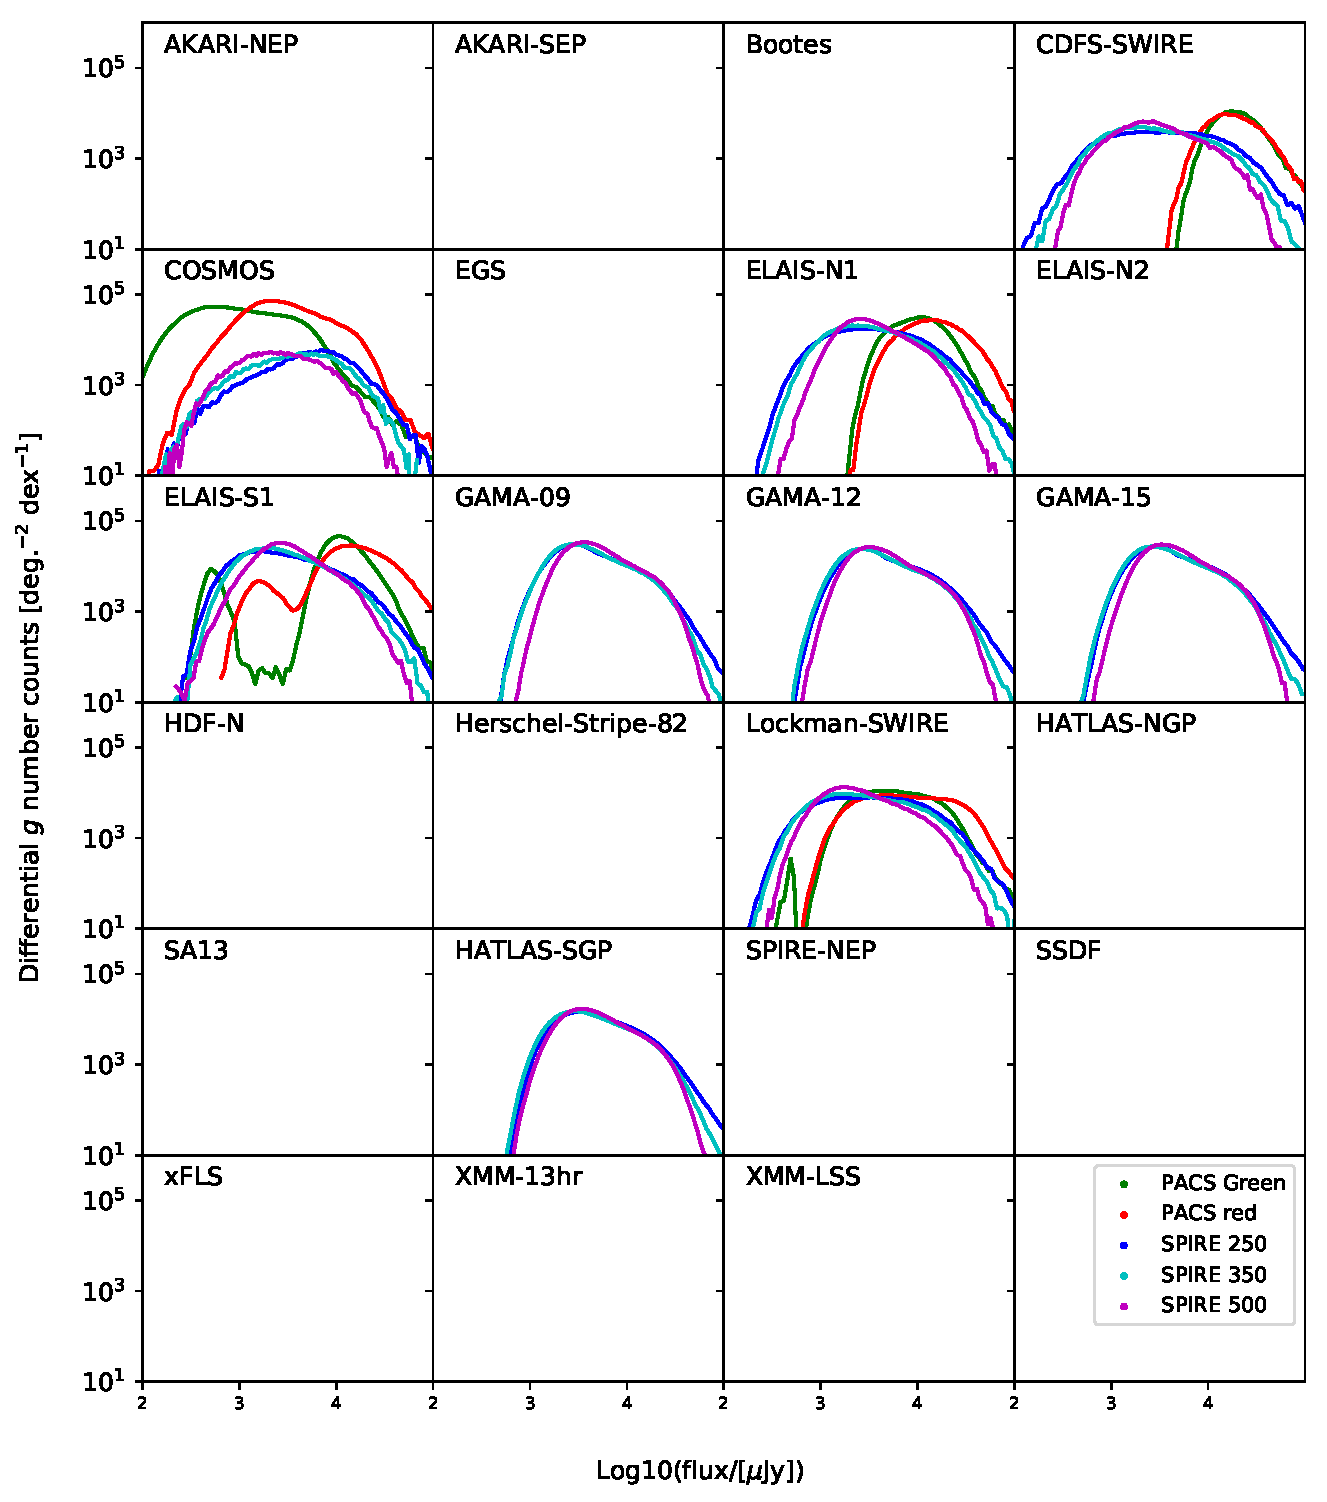
\includegraphics[width=1.0\textwidth]{./figs/numbers_Herschel_allfields}
\caption{\label{fig:numbers_allfields} The differential number counts in Herschel bands on each field. {\color{red} RERUN AFTER ALL FIELDS DONE. DO THESE LOOK OK?????}   }
\end{figure*}

\subsection{Summary of master list}
\subsection{Summary of priors}
\subsection{Summary of XID+ catalogues}

\subsection{Monochromatic depth maps, area vs 1-sigma depths for catalogues}

Figure~\ref{fig:bands_depths} shoes an overview of depths for each band compared to typical galaxy SEDs. {\color{red} ALSO INCLUDE some two d depth historgrams MIPS vs R???, RAPH NEEDS TO MAKE DEPTH MAPS FOR MIPS/PACS/SPIRE to make these figures. Also add deepest ugrizyJHKKs columns!!!}.

\begin{figure*}
\centering
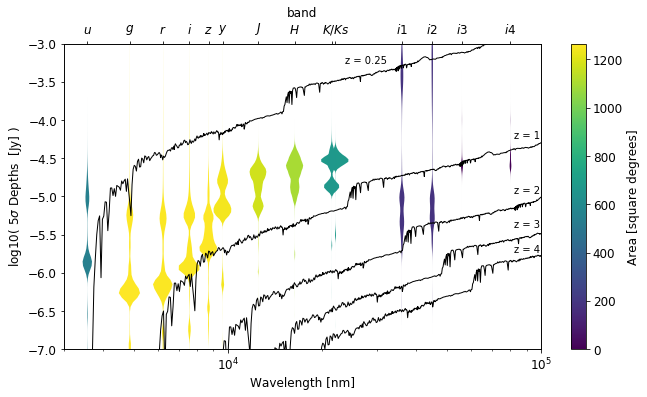
\includegraphics[width=0.9\textwidth]{./figs/band_depths_overviews_areaweighted_with_black_seds_wave}
\caption{\label{fig:bands_depths}{\color{red} FIGURE FROM SHIRLEY ET AL BUT WITH MIPS PACS AND SPIRE TO BE ADDED!!!}The distribution of $5\sigma$ point-source depths in a 2 arcsec aperture for each broad band type (taking the deepest specific band available in a given HEALPix cell). The colour of each area is determined by the total area that data for that band is available. The areas of each probability density function are also weighted by the total area available for that band so that area in a given curve is proportionally related to area on the sky that a given band is available at a given depth. The combination of areas covered by either the $K$ or $K_s$ bands is the full 1270 deg.$^2$ of HELP. We also plot a typical HELP spectral energy distribution for a galaxy with star formation rate of 200~M$_\odot$/yr and a stellar mass of $10^{10}$~M$_\odot$ at various redshifts.}
\end{figure*}





\subsection{Monochromatic Completeness limits }

\subsection{di-chromatic and multi-chromatic depths?}

\subsection{number counts}
{\color{red} a per field full page figure as in Shirley et al with spire 250,350, 500 number counts?}


\section{Extra section}

\subsection{P-value map sources (probably not)?}
\subsection{Red objects}

\section{Discussion and Conclusion}

\subsection{To include a section on science that is being done with this data set now}


\subsection{Examples of tools}

\subsection{How people can contribute}


To summarise: 

\begin{itemize}
\item We present forced far-infrared photometry over 1270 deg.$^2$ of prime extragalactic fields imaged by the \emph{Herschel} Space observatory. We calculate a posterior on the flux for all objects in a simply defined prior list chosen to be tightly correlated with far-infrared bright objects using Bayesian inference. 
\item We present photometric redshifts, and physical properties calculated using spectral energy distribution modelling for XXX objects, chosen using a simple well defined selection function. 
\item This new catalogue is presented alongside an array of other data products, including newly homogenised maps, supplementary catalogues and extensive tools for accessing these new data sets.
\end{itemize}

%%%%%%%%%%%%%%%%%%%%%%%%%%%%
% BIBLIOGRAPHY


\section*{Data used in this paper}

The catalogue described in this paper is available at \url{hedam.lam.fr/HerMES}



\section*{Acknowledgements}

%Charlotte Clarke acknowledges support from the Science and Technology
%Facilities Council (grant number ST/J50077X/1)

The research leading to these results has received funding from the European
Union Seventh Framework Programme FP7/2007-2013/ under grant agreement No.
607254.


Seb Oliver acknowledges support from the Science and Technology Facilities
Council (grant number ST/L000652/1)


HCSS / HSpot / HIPE are joint developments by the Herschel Science Ground
Segment Consortium, consisting of ESA, the NASA Herschel Science Center, and the
HIFI, PACS and SPIRE consortia.

This research has found TOPCAT \citep{2005ASPC..347...29T} extremely useful.

This research has made use of the NASA/IPAC Extragalactic Database (NED) which
is operated by the Jet Propulsion Laboratory, California Institute of
Technology, under contract with the National Aeronautics and Space
Administration.

SPIRE has been developed by a consortium of institutes led by Cardiff Univ. (UK)
and including Univ. Lethbridge (Canada); NAOC (China); CEA, LAM (France); IFSI,
Univ. Padua (Italy); IAC (Spain); Stockholm Observatory (Sweden); Imperial
College London, RAL, UCL-MSSL, UKATC, Univ. Sussex (UK); Caltech, JPL, NHSC,
Univ. Colorado (USA). This development has been supported by national funding
agencies: CSA (Canada); NAOC (China); CEA, CNES, CNRS (France); ASI (Italy);
MCINN (Spain); SNSB (Sweden); STFC, UKSA (UK); and NASA (USA).

HELP would like to thank the HELP Scientific Advisory Board members past and
present for invaluable advice in the defining of the project: Simon Driver,
Loretta Dunne, Carol Lonsdale, Mark Lacy, Peter Capak, Takashi Onaka, Mara
Salvato, Brent Groves, G\"{o}ran Pilbratt, David Elbaz

Huge thanks also to our Project Manager, Louise Winters, for keeping us on-track
and on-time with good humour.

The data presented in this paper is released through the {\em Herschel} Database
in Marseille HeDaM ({\url{http://hedam.lam.fr/HerMES}})

\bibliography{./HELP_bib}

%%%%%%%%%%%%%%%%%%%%%%%%%%%%


%%%%%%%%%%%%%%%%%%%%%%%%%%%%
% START APPENDICES
\appendix


% \section{HeDAM standards}\label{sec:standards}

% Only needed if we are going to publish these, maybe even they are obsolete now?

\section[Multi-wavelength Survey Audit\\{\color{red}Obsolete?}]{Multi-wavelength Survey Audit}

In this section we briefly summarise the data that is anticipated to be included
in HELP.   The summaries are grouped into broad wavelength regions over which
the properties are similar. We also highlight any specific value that HELP
expects to add to these data.

\subsection{X-ray}

\subsection{UV}

\subsection{Optical}

\subsection{NIR: 1-3\micron}

The whole of HELP is of course covered by the 2MASS survey and this data set
provides us with a key astrometric reference and a homogeneous catalogue of
sizes.  In the  near infrared the primary data products that are available are
the UKIRT and VISTA public surveys.  These overlap with most of the survey
fields. A few of the fields are substantially better covered by other surveys.
In Table~\ref{tab:k} we summarise the specific surveys that are currently
expected to be included in HELP.  Using our depth maps (see e.g.
Figure~\ref{fig:k}) we have also estimated the area in deg.$^2$ that are covered
above a few (arbitrary) $K_{\rm AB}$ limits to give some idea of the coverage.

These wavebands form a primary source for our master lists and thus drive the
selection functions.

The key value that will be added by HELP at these wavelengths is consistent
photometry extracted where necessary from the original survey images.

% \begin{table*}
%   \begin{tabular}{|l|r|r|l|r|r|r|r|l|}
\hline
  \multicolumn{1}{|c|}{Name} &
  \multicolumn{1}{c|}{RA} &
  \multicolumn{1}{c|}{Dec} &
  \multicolumn{1}{c|}{Key Data} &
  \multicolumn{1}{c|}{$K_{\rm AB}>23.7$} &
  \multicolumn{1}{c|}{$K_{\rm AB}>22$} &
  \multicolumn{1}{c|}{$K_{\rm AB}>20.75$} &
  \multicolumn{1}{c|}{$K_{\rm AB}>19.5$} &
  \\
\hline
  SSDF & -8.1 & -55.114 & VISTA-VHS &  & 9.7 & 45.0 & 105.0 & \\
  HATLAS-SGP & 1.5 & -32.734 & VISTA-VHS &  & 7.3 & 292.0 & 294.0 & \\
  ELAIS-S1 & 8.8 & -43.585 & VISTA-VIDEO & 2.8 & 2.8 & 3.4 & 8.9 & \\
  Herschel-Stripe-82 & 14.3 & -0.034 & VISTA-VHS &  & 7.5 & 86.2 & 374.0 & \\
  XMM-LSS & 35.1 & -4.528 & VISTA-VIDEO & 1.0 & 10.5 & 13.2 & 21.5 & \\
  CDFS-SWIRE & 53.1 & -28.235 & VISTA-VIDEO & 2.6 & 4.6 & 8.7 & 12.0 & \\
  AKARI-SEP & 70.8 & -53.862 & VISTA-VHS &  &  & 1.7 & 7.3 & \\
  GAMA-09 & 134.7 & 0.513 & VISTA-VIKING &  & 0.4 & 56.2 & 61.2 & \\
  COSMOS & 150.1 & 2.218 & VISTA-ULTRAVISTA & 1.0 & 1.0 & 1.2 & 5.0 & \\
  Lockman-SWIRE & 161.2 & 58.058 & UKIDS-DXS &  & 10.4 & 10.5 & 10.8 & \\
  GAMA-12 & 179.8 & -0.482 & VISTA-VIKING &  & 3.1 & 59.0 & 61.9 & \\
  HDF-N & 189.2 & 62.241 & Various &  &  &  &  & \\
  SA13 & 198.0 & 42.715 & ? & 0.2 & 0.2 & 0.2 & 0.2 & \\
  HATLAS-NGP & 199.5 & 29.215 & UKIDS-LAS &  & 18.1 & 62.1 & 179.0 & \\
  XMM-13hr & 203.6 & 37.918 & ? &  & 0.7 & 0.7 & 0.7 & \\
  EGS & 215.0 & 52.72 & ? &  & 0.1 & 0.7 & 0.7 & \\
  GAMA-15 & 217.6 & 0.456 & VISTA-VIKING &  & 1.2 & 60.2 & 60.9 & \\
  Bo\"otes & 218.1 & 34.173 &  &  & 4.9 & 5.2 & 5.2 & \\
  ELAIS-N1 & 242.9 & 55.071 & UKIDS-DXS &  & 9.4 & 9.8 & 9.9 & \\
  ELAIS-N2 & 249.2 & 41.058 & UKIDS-LAS &  & 0.1 & 0.2 & 0.8 & \\
  xFLS & 259.0 & 59.384 & UKIDS-LAS &  & 0.1 & 2.6 & 2.7 & \\
  SPIRE-NEP & 265.0 & 69.004 & UKIDS-LAS &  &  &  &  & \\
  AKARI-NEP & 270.0 & 66.556 & UKIDS-LAS &  &  &  &  & \\
  Total	&	&	&	& 7.6	&92.1	&718.8	&1221.7\\
\hline\end{tabular}

%   \caption{Audit of data in near infra-red bands}\label{tab:k}
% \end{table*}

% \subsection{Mid-IR: 3.6-12\micron}

% \subsection{FIR: 24-500\micron}

% \subsection{sub-mm}

% \subsection{Radio}

% \subsection{Spectroscopic Redshifts}

\section{OBSIDS}

This Appendix lists the OBSIDS used in HELP

HELP comprises the  Herschel OBSIDS: 1342257362, 1342247216,
1342246632, 1342246580, 1342238251, 1342237563, 1342237553, 1342237550,
1342236240, 1342236234,1342236232, 1342234749.

All products available through the HELP www pages \url{herschel.sussex.ac.uk}.


\section{Database structure and access}


DMU0	Pristine catalogues
DMU1	Masterlist data
DMU2	Field definitions
DMU3	Morphologies (under development)
DMU4	Bright Star Mask
DMU5	Known Star Flag
DMU6	Optical photometry validation
DMU7	Optical photometry (under development)
DMU8	Radio data - LOFAR & FIRST/NVSS/TGSS
DMU9	Radio data - JVLA-DEEP & GMRT-DEEP
DMU10	Data Fusion
DMU11	Cross matching MIPS/PACS/SPIRE (under development)
DMU12	Cross Matching LOFAR & FIRST/NVSS/TGSS
DMU13	Cross Matching JVLA-DEEP & GMRT-DEEP
DMU14	GALEX data
DMU15	X-Ray data (under development)
DMU16	WISE Photometry
DMU17	MIPS Maps
DMU18	PACS maps
DMU19	SPIRE maps
DMU20	MIPS blind photometry (under development)
DMU21	PACS blind photometry (under development)
DMU22	SPIRE blind photometry
DMU23	Spec-z data
DMU24	Photo-z
DMU25	Prior model
DMU26	XID+
DMU27	Empirical models / templates (under development)
DMU28	SED fitting / CIGALE
DMU29	Radiative transfer models (under development)
DMU30	Missing (supplementary) Sources (under development)
DMU31	Tools
DMU32	Merged catalogue


%%%%%%%%%%%%%%%%%%%%%%%%%%%%

%%%%%%%%%%%%%%%%%%%%%%%%%%%%
% END DOCUMENT
\end{document}
%%%%%%%%%%%%%%%%%%%%%%%%%%%%
